% PLANTILLA APA7
% Creado por: Isaac Palma Medina
% Última actualización: 25/07/2021
% @COPYLEFT

% Fuentes consultadas (todos los derechos reservados):  
% Normas APA. (2019). Guía Normas APA. https://normas-apa.org/wp-content/uploads/Guia-Normas-APA-7ma-edicion.pdf
% Tecnológico de Costa Rica [Richmond]. (2020, 16 abril). LaTeX desde cero con Overleaf (1 de 3) [Vídeo]. YouTube. https://www.youtube.com/watch?v=kM1KvHVuaTY Weiss, D. (2021). 
% Formatting documents in APA style (7th Edition) with the apa7 LATEX class. https://ctan.math.washington.edu/tex-archive/macros/latex/contrib/apa7/apa7.pdf @COPYLEFT

%+-+-+-+-++-+-+-+-+-+-+-+-+-++-+-+-+-+-+-+-+-+-+-+-+-+-+-+-+-+-++-+-+-+-+-+-+-+-+-+

% Preámbulo
\documentclass[stu, 12pt, letterpaper, donotrepeattitle, floatsintext, natbib, helv]{apa7}
\usepackage[utf8]{inputenc}
\usepackage{comment}
\usepackage{marvosym}
\usepackage{graphicx}
\usepackage{float}
\usepackage[normalem]{ulem}
\usepackage[spanish]{babel} 
%\usepackage{titling}
\let\apasubparagraph\subparagraph
\let\subparagraph\paragraph
\usepackage[compact]{titlesec}
\let\subparagraph\apasubparagraph
\usepackage{hyperref}
\selectlanguage{spanish}
\useunder{\uline}{\ul}{}
\newcommand{\myparagraph}[1]{\paragraph{#1}\mbox{}\\}
\graphicspath{{./images/}}
\titleformat{\section}{\normalfont\large\bfseries}{\thetitle. \quad }{0pt}{}[{ \titlerule[0.8pt]}]
\titleformat{\subsection}{\normalfont\bfseries}{}{}{}[]

% Portada

\begin{document}
\begin{titlepage}
    \centering
    \vfill
    \LARGE Laboratorio \#4\\
    \vskip2cm
    \large Diego Quirós Artiñano \\
    Universidad Nacional de Costa Rica \\
    EIF-202: Soporte Técnico \\ 
    Carolina Gómez Fernández \\
    24 de abril, 2022 \\
    \vfill
    
\includegraphics[width = 0.4\textwidth]{../../../UNAImage/UNA.png} \\
    \vfill
    \vfill
    % (autores separados, consultar al docente)
    % Manera oficial de colocar los autores:
    %\author{Autor(a) I, Autor(a) II, Autor(a) III, Autor(a) X}
\end{titlepage}

% Índices
\pagenumbering{roman}
    % Contenido
\addto\captionsspanish{
    \renewcommand*\contentsname{\largeÍndice}
}
\tableofcontents
\setcounter{tocdepth}{2}
\newpage
    % Figuras
\renewcommand{\listfigurename}{\largeÍndice de fíguras}
\listoffigures
\newpage
    % Tablas
\renewcommand{\listtablename}{\largeÍndice de tablas}
\listoftables
\newpage

% Cuerpo
\pagenumbering{arabic}

%------------------------------------------------------------------------------------
\section*{Introducción}
\phantomsection
\addcontentsline{toc}{section}{Introducción}

En este documento se van a ver varios aspectos de las tarjetas madre, se van a ver el chipset, BIOS y códigos de error.
%------------------------------------------------------------------------------------
\section*{Chipset}
\phantomsection
\addcontentsline{toc}{section}{Chipset}

\begin{enumerate}
    \item Identificar mediante el software el chipset:
    \begin{figure}[H]
        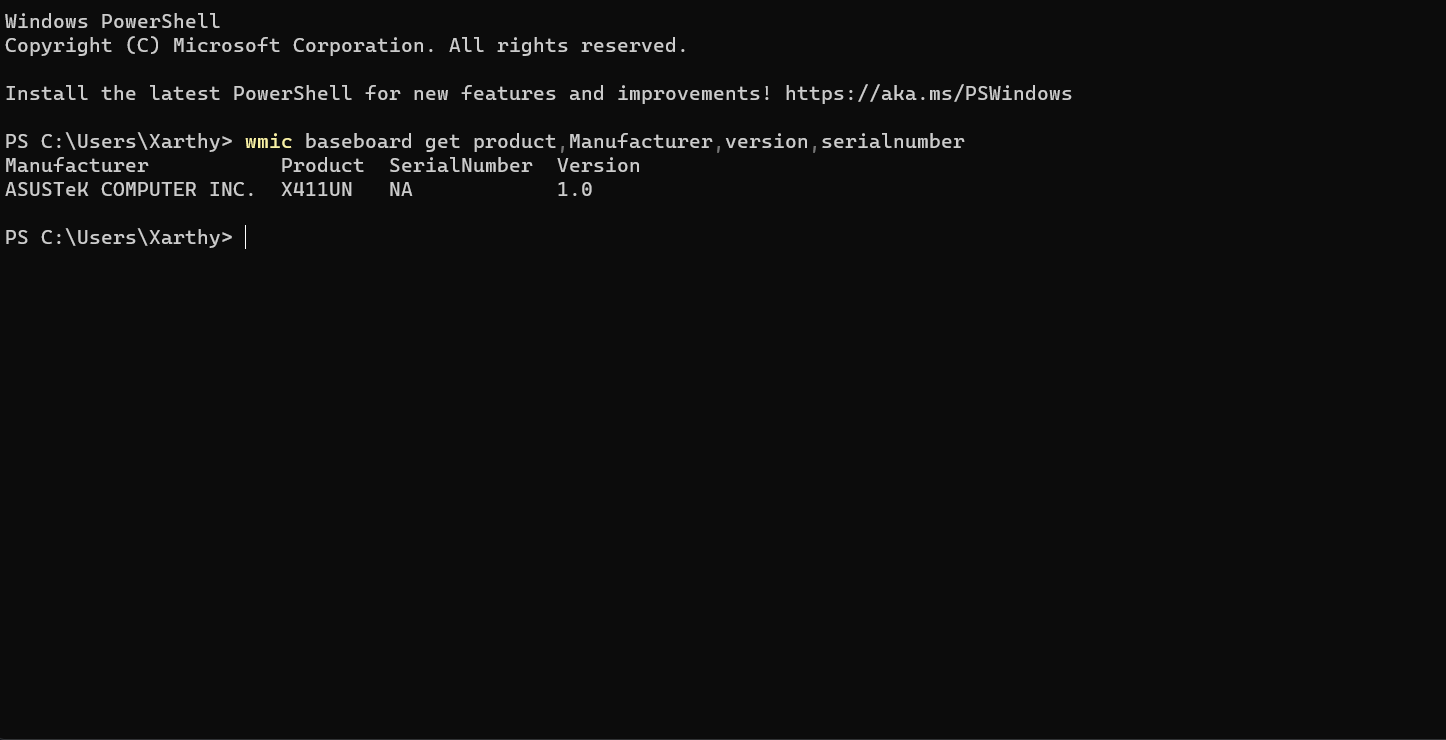
\includegraphics[width=1\textwidth]{wmic_cmd_details.png}
        \caption{Chipset a través del cmd}
        \label{fig:cmdFig}
    \end{figure}
    \item Identificar el chipset mediante programas terceros y ¿Cuáles datos encontró sobre el chipset?
    \begin{figure}[H]
        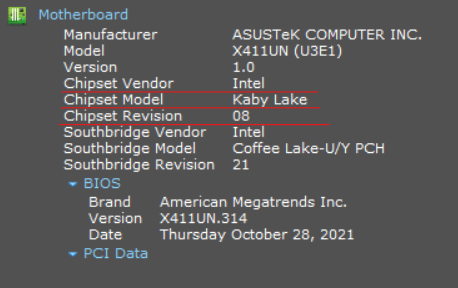
\includegraphics[width=0.9\textwidth]{Speccy.png}
        \caption{Chipset a través de Speccy}
        \label{fig:speccyFig}
    \end{figure}
\end{enumerate}

%------------------------------------------------------------------------------------
\section*{BIOS}
\phantomsection
\addcontentsline{toc}{section}{BIOS}

\begin{enumerate}
    \item Identifique las teclas para ingresar al BIOS en su computadoras (anótelas): Las teclas esc sirve para entrar al bootloader desde el cual se puede ingresar al BIOS a través de la opción Setup. La tecla f2 ingresa directamente al BIOS.
    \item ¿Quién es el fabricante del BIOS?: ASUS
    \item ¿Cuál es la versión del BIOS?: 314, GOP: 9.0.1066, EC:F0KL2091.009
    \item Identifique la tarjeta madre y busque en Internet cual es la versión más actualizada de BIOS para esa tarjeta. La Tarjeta Madre es: ASUSTek COMPUTER INC. X411UN (U3E1) y la versión más reciente del BIOS es 314 (está actualizada). 
\end{enumerate}

%------------------------------------------------------------------------------------
\section*{Simulador BIOS}
\phantomsection
\addcontentsline{toc}{section}{Simulador BIOS}

\begin{enumerate}
    \item Ingrese a https://geekprank.com/bios/
    \item Liste las opciones del menú principal
    \begin{itemize}
        \item System Time
        \item System Date
        \item Primary IDE Master
        \item Primary IDE Slave
        \item SATA1
        \item SATA2
        \item SATA3
        \item SATA4
        \item Storage Configuration
        \item System Information
    \end{itemize}
    \item Busque en las pantallas para ubicar la información del CPU
    \item ¿Qué información de la CPU se incluye?
    \begin{itemize}
        \item CPU Type; Intel (R) Core(TM)2 Quad CPU Q66 @ 2.40GHz
        \item CPU Speed: 2.40GHz/1066MHz
    \end{itemize}
    \item Explore cada pantalla en busca de la configuración de la RAM.
    \item ¿Cuál es la velocidad de la RAM?: 1066MHz, está es la velocidad del bus y es en la que el RAM depende de.
    \item ¿Qué otra información de la RAM se incluye?: Cache RAM: 8192KB
    \item Explore cada pantalla en busca de la configuración del disco duro.
    \item ¿Qué información del disco duro se incluye?:
    \begin{itemize}
        \item Hay dos SATAs configurados, uno en el SATA1 que es un HL-DT-ST DVDRW GH, el otro está en el SATA2 que es un SAMSUNG HD103SJ
    \end{itemize}
    \item Explore cada pantalla en busca de la secuencia del orden de arranque.
    \item ¿Cuál es el primer dispositivo de arranque en la secuencia del orden de arranque?: el primer dispositivo en el orden de arranque (boot order) es el WCD WD1600BEVT-223CHG-(PM)
    \item ¿Cuántos dispositivos adicionales pueden asignarse en la secuencia del orden de arranque?: Hay 6 dispositivos adicionales: 
    \begin{itemize}
        \item CD/DVD: Optiarc: DVD RW AD-98123-(P)
        \item Network Boot: MBA v11.0.11 Slot 0200
        \item USB HDD
        \item USB FDD
        \item USB KEY
        \item USB CD/DVD ROM
    \end{itemize}
    \item Indique como cambiar el orden de arranque: El BIOS normalmente tendrá indicaciones para decir como hacer cosas en algún lugar de la pantalla, que teclas usar, por ejemplo en el BIOS de mi computadora es ingresar como cualquier sub-menú y seleccionar el dispositivo de boot que quiera, o generar un nuevo boot load. En este BIOS del ejemplo es un Phoenix-BIOS entonces lo tuve que buscar, según \cite{BIOSBootChanges} se utilizan las teclas + y - para cambiarle el orden y después de hacer todos los cambios deseados se salvan los cambios con la tecla indicada abajo o quit without saving en el caso que no se quiera salvar.
\end{enumerate}

%------------------------------------------------------------------------------------
\section*{Códigos de error}
\phantomsection
\addcontentsline{toc}{section}{Códigos de error}

Aunque no encontrara específicamente para mi BIOS, encontré un artículo que menciona generalmente los códigos que se usan.

\begin{table} [H]
    \centering
    \begin{tabular}{|p{4cm} | p{11cm}|}
        \hline
        Código & Significado \\
        \hline\hline
        1 beep corto & Fallo de refrescamiento de DRAM (\textit{DRAM refresh failure}) \\
        \hline
        2 beeps cortos & Fallo de paridad de circuito (\textit{Parity circuit failure}) \\
        \hline 
        3 beeps cortos & Fallo de base 64 K RAM (\textit{Base 64 K RAM failure}) \\
        \hline
        4 beeps cortos & Fallo de reloj de sistema (\textit{System timer failure}) \\
        \hline
        5 beeps cortos & Fallo de proceso (\textit{Process failure}) \\
        \hline
        6 beeps cortos & Error de puerta A20 de controlador de teclado (\textit{Keyboard controller Gate A20 error}) \\ 
        \hline
        7 beeps cortos & Error de excepción de modo virtual (\textit{Virtual mode exception error}) \\
        \hline
        8 beeps cortos & Fallo de memoria de display Lectura y Escritura (\textit{Display memory Read/Write test failure}) \\
        \hline
        9 beeps cortos & Fallo de ROM BIOS (\textit{ROM BIOS checksum failure}) \\
        \hline
        10 beeps cortos & Error de batería CMOS (\textit{CMOS battery error}) \\
        \hline
        11 beeps cortos & Error de memoria de Cache (\textit{Cache memory error}) \\
        \hline
        1 beeps largos + 3 cortos & Fallo de memoria extendida o convencional (\textit{Conventional or Extended memory failure}) \\
        \hline
        1 beeps largos + 8 cortos & Fallo de prueba de display/retrace (\textit{Display/Retrace test failed)}) \\
        \hline
        Two-tone siren & Velocidades bajas de abanico de CPU o niveles de voltaje (\textit{Low CPU fan speed, or voltage level issue)}) \\
        \hline
    \end{tabular}
    \caption{Códigos de errores de ASUS, según \cite{ErrorCodes}}
    \label{tab:errorsTable}
\end{table}
%Encontrar los errores de mi BIOS y modificar tabla
%----------------------------------------------------------------------------------------------------------------------------------------------------------------------
\section*{Conclusión}
\phantomsection
\addcontentsline{toc}{section}{Conclusión}
En este laboratorio se investigó sobre el Chipset de mi computadora y sus especificaciones. Siguiente se investigó sobre el BIOS de mi computadora sus especificaciones y si estaba al día. Siguiente se usó un simulador para ver como encontrar información de las computadoras y como cambiarle el orden de arranque. Finalmente, se buscaron los códigos de error básicos de BIOS según el fabricante de mi computadora (ASUS).

\newpage
% Referencias
\renewcommand\refname{\large\textbf{Referencias}}
\bibliography{ref}

\end{document}